\documentclass{article}
\usepackage{tikz}
\usepackage{pgfplots}
\begin{document}

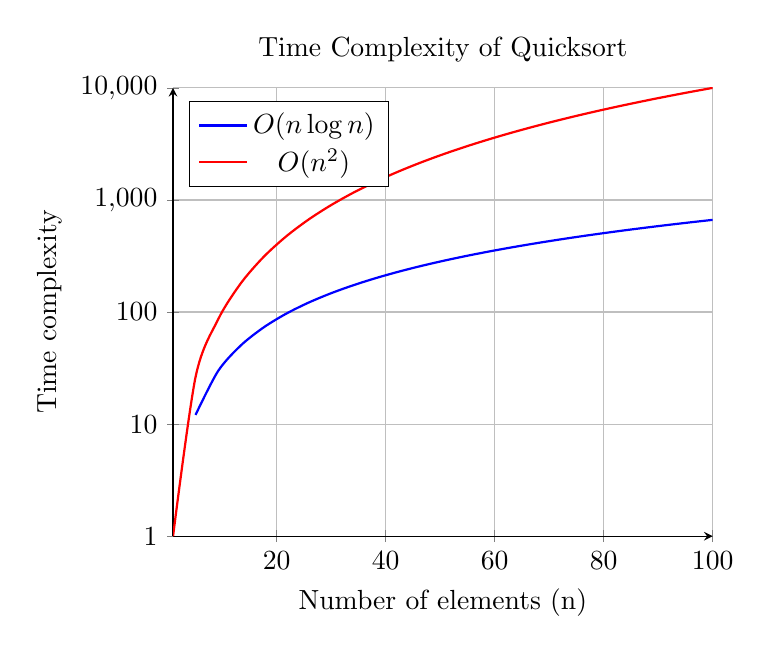
\begin{tikzpicture}
\begin{axis}[
    title={Time Complexity of Quicksort},
    xlabel={Number of elements (n)},
    ylabel={Time complexity},
    domain=1:100,
    legend pos=north west,
    ymode=log,
    log basis y={2},
    ymin=1,
    ymax=10000,
    xtick={0,20,40,60,80,100},
    ytick={1,10,100,1000,10000},
    log ticks with fixed point,
    axis lines = left,
    grid=both,
    smooth
]
% Average and Best Case O(n log n)
\addplot [
    thick,
    color=blue,
] {x*log2(x)};
\addlegendentry{\(O(n \log n)\)}

% Worst Case O(n^2)
\addplot [
    thick,
    color=red,
] {x^2};
\addlegendentry{\(O(n^2)\)}
\end{axis}
\end{tikzpicture}

\end{document}
